% !TeX root = ../tfg.tex
% !TeX encoding = utf8

\chapter{Trabajos relacionados}\label{sec:evolucion-ddd}

El \emph{Deep Double Descent}, al estar estrechamente relacionado al avance tecnológico y al crecimiento en la capacidad y el tamaño de los modelos de aprendizaje profundo, ha despertado un mayor interés en los últimos años, como puede observarse en la~\autoref{fig:histogram}. No obstante, aunque se percibe durante los últimos años una tendencia al alza del número de artículos que hacen referencia al mismo, únicamente encontramos un total $224$ publicaciones en Scopus\footnote{Encontradas $224$ publicaciones a fecha $21$ de marzo de $2025$ usando la consulta:  
\texttt{TITLE-ABS-KEY ((deep AND double AND descent) OR (overparameterized AND generalization)) AND PUBYEAR < 2025 AND (LIMIT-TO (SUBJAREA,\textquotedblleft COMP\textquotedblright) OR LIMIT-TO (SUBJAREA,\textquotedblleft ENGI\textquotedblright) OR LIMIT-TO (SUBJAREA,\textquotedblleft MATH\textquotedblright) OR LIMIT-TO (SUBJAREA,\textquotedblleft PHYS\textquotedblright)) AND (LIMIT-TO (EXACTKEYWORD,\textquotedblleft Machine Learning\textquotedblright) OR LIMIT-TO (EXACTKEYWORD,\textquotedblleft Deep Learning\textquotedblright) OR LIMIT-TO (EXACTKEYWORD,\textquotedblleft Generalization\textquotedblright) OR LIMIT-TO (EXACTKEYWORD,\textquotedblleft Performance\textquotedblright) OR LIMIT-TO (EXACTKEYWORD,\textquotedblleft Neural-networks\textquotedblright) OR LIMIT-TO (EXACTKEYWORD,\textquotedblleft Deep Neural Networks\textquotedblright) OR LIMIT-TO (EXACTKEYWORD,\textquotedblleft Overparameterization\textquotedblright) OR LIMIT-TO (EXACTKEYWORD,\textquotedblleft Overfitting\textquotedblright) OR LIMIT-TO (EXACTKEYWORD,\textquotedblleft Generalization Error\textquotedblright) OR LIMIT-TO (EXACTKEYWORD,\textquotedblleft Generalization Performance\textquotedblright) OR LIMIT-TO (EXACTKEYWORD,\textquotedblleft Neural Networks\textquotedblright) OR LIMIT-TO (EXACTKEYWORD,\textquotedblleft Interpolation\textquotedblright) OR LIMIT-TO (EXACTKEYWORD,\textquotedblleft Generalize\textquotedblright))}.}. Esta reciente relevancia ilustra el carácter \textbf{innovador} y \textbf{pionero} de este proyecto.\newline

\begin{figure}[h]
    \centering
    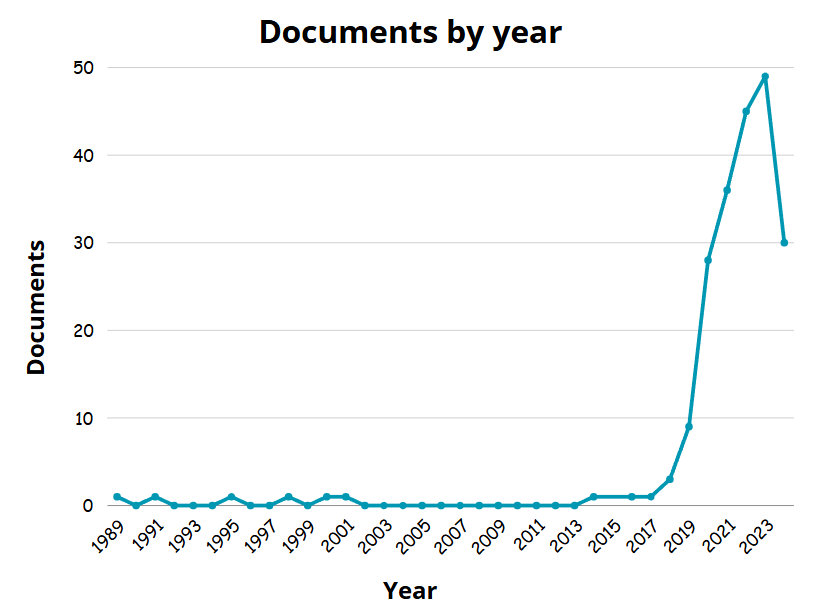
\includegraphics[width=0.8\linewidth]{img/scopus_histogram.png}
    \caption[Número de publicaciones relativas al \textit{Deep Double Descent} (ir actualizando histograma de cara a nuevos papers).] {Número de publicaciones relativas al \textit{Deep Double Descent} en función del año de publicación.}\label{fig:histogram}
\end{figure}

Sin embargo, aunque la cantidad de artículos científicos aún sea limitada, el interés por parte de investigadores y científicos está creciendo rápidamente. Incluso en ausencia de publicaciones científicas formales, se continúan obteniendo nuevos resultados, tanto teóricos como prácticos, que continúan enriqueciendo nuestra comprensión del problema.\newline

A pesar de la disponibilidad de artículos que abordan el tema, la mayoría de ellos no proporcionan una explicación detallada del mismo, centrándose generalmente en casos prácticos y dejando de lado el análisis teórico intrínseco, limitando su comprensión completa.\newline

\section{Origen y primeras manifestaciones}\label{}

Aunque la primera publicación sobre el \textit{Deep Double Descent} se remonta a $1998$, como se observa en la Figura~\ref{fig:histogram}, comportamientos similares parecen haber sido descritos por primera vez en la literatura de la física teórica en $1989$, siendo esta la primera publicación formal.\newline

En ese año, Vallet et al.~\cite{Vallet1989} presentaron, de manera empírica, esta dinámica al emplear la pseudoinversa para abordar problemas de regresión lineal con datos artificiales. La siguiente evidencia empírica fue presentada por Krogh \& Hertz en el año $1991$~\cite{Krogh1991}, quienes, de manera parcial, mostraron el suceso utilizando un modelo de regresión lineal.\newline

Posteriormente, nos remontamos hasta $1995$ cuando Opper presenta los primeros resultados teóricos en su artículo ``Statistical Mechanics of Generalization''~\cite{Opper1995}, a través del uso de una red neuronal formada por un perceptrón de una sola capa con una función de activación lineal conocida como ADALINE~\cite{WidrowHoff1960}, y, más tarde, en su revisión del artículo en $2001$ ``Learning to Generalize''~\cite{Opper2001}.\newline

\begin{figure}[h]
    \centering
    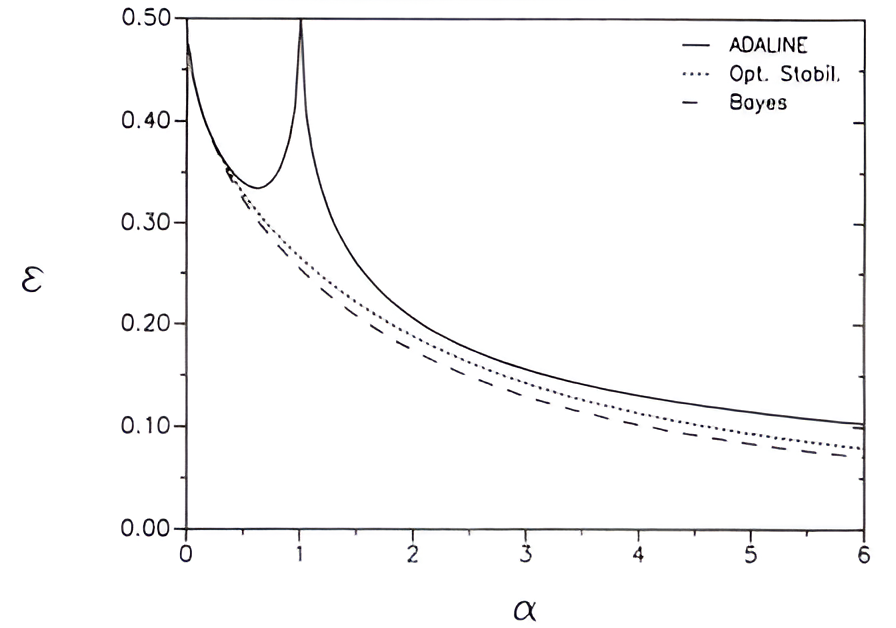
\includegraphics[width=0.8\linewidth]{img/estadoarte2.png}
    \caption[Deep Double Descent presente en ADALINE.]{Comparación del error de generalización ($\epsilon$) para distintos modelos en función de la fracción entre el número de ejemplos aprendido y el número de parámetros ($\alpha$). Se observa la curva del doble descenso para el modelo ADALINE~\cite{Opper1995}.}\label{fig:estadoarte2}
\end{figure}

En sus representaciones (véase~\autoref{fig:estadoarte2}), el error de generalización ($\epsilon$) se muestra en función del número de ejemplos de entrenamiento ($n$) y el número de parámetros ($P$), donde $\alpha = \frac{n}{P}$. Se observa que el error de generalización alcanza su máximo cuando $\alpha$ se aproxima a $1$, es decir, cuando el número de ejemplos de entrenamiento es similar al número de parámetros del modelo. En adición, demuestra que, para ciertas configuraciones, cuando $N$ tiende a infinito, la solución que proporciona la pseudoinversa mejora a medida que nos alejamos del ``pico'' $(\alpha = 1)$. \newline

Comportamientos similares a los obtenidos por Opper también han sido reportados por Advani \& Saxe en $2017$~\cite{Advani2017}, así como por Spigler et al.\ y Geiger et al.\ en $2019$~\cite{Spigler2019, Geiger2019}. Estos trabajos, anteriores a la formalización del fenómeno tal como se conoce hoy en día, trabajan con redes neuronales profundas con un gran número de parámetros y estudian el comportamiento del error de generalización utilizando herramientas de física estadística inspiradas en el trabajo de Opper. De esta manera, Spigler et al.\ y Geiger et al.\ proponen una conexión entre el doble descenso y la transición \textit{jamming} propia de la física estadística, mostrando por qué los modelos pueden llegar a generalizar mejor después del ``pico'' del error de prueba.\newline

No obstante, fue Duin en el año $2000$~\cite{Duin2000} (véanse Figuras 6 y 7) el primero en mostrar curvas de generalización utilizando datos del mundo real, bastante similares a las curvas del doble descenso que tenemos hoy en día.\newline

\section{El nacimiento del Deep Double Descent}\label{}

Iniciamos esta sección abordando el equilibrio clásico entre sesgo y varianza, un concepto fundamental en la teoría del aprendizaje automático~\cite{Geman1992, Hastie2001, Bengio2010}. Esta teoría sostiene que, a medida que la complejidad de un modelo aumenta, su sesgo disminuye, pero su varianza se incrementa. Como resultado, llega un punto en el que el error de generalización aumenta, formando la tradicional curva en forma de ``U''. De acuerdo con esta visión tradicional, una vez superado cierto umbral de complejidad, los modelos más grandes son cada vez peores y, por tanto, se busca encontrar un equilibrio en el modelo.\newline

Sin embargo, los resultados prácticos modernos no comparten esta teoría. En la actualidad, la visión moderna entre los profesionales es que los \emph{modelos grandes son mejores}~\cite{Krizhevsky2012, Neal2019, Huang2019, Szegedy2014}. Estos estudios muestran que el uso de redes neuronales con un gran número de parámetros conduce a un mejor rendimiento, evidenciando que los modelos más complejos pueden obtener resultados superiores a los modelos simples.\newline

Este trabajo se enmarca dentro del estudio de la generalización en redes neuronales profundas. En particular, se enlaza con investigaciones previas, como la de Zhang et al.\ en $2021$~\cite{Zhang2021}, quienes argumentan que comprender el aprendizaje profundo aún requiere replantearse los paradigmas tradicionales de generalización, desafiando la noción clásica de sesgo-varianza.\newline

El \emph{Deep Double Descent} fue nombrado así, por primera vez, por Belkin et al.\ en $2019$ \cite{Belkin2019}, haciendo referencia a los dos descensos que presenta la curva del error de generalización. En este artículo, se busca unificar la teoría clásica del equilibrio sesgo-varianza con los resultados prácticos obtenidos por la teoría moderna, mediante una curva de error unificada (véase~\autoref{fig:estadoarte2.2}).\newline

\begin{figure}[h]
    \centering
    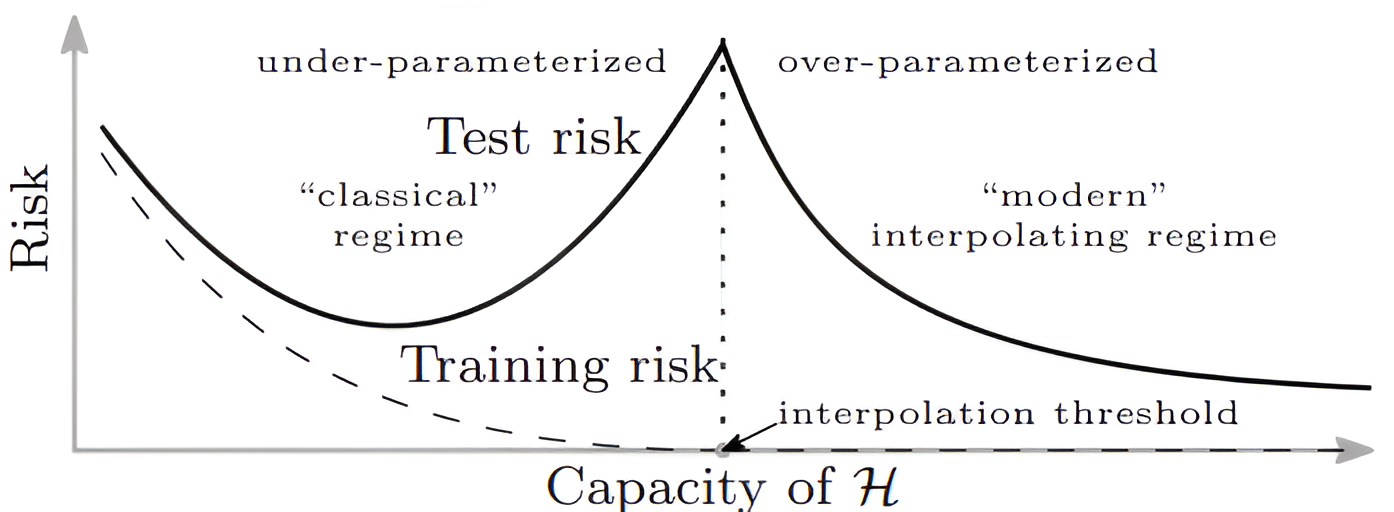
\includegraphics[width=0.8\linewidth]{img/estadoarte2.2.png}
    \caption[Curva del error unificada entre la teoría clásica y moderna~\cite{Belkin2019}.]{Curvas para el error de entrenamiento (línea discontinua) y el error de generalización (línea continua)~\cite{Belkin2019}. Antes del umbral de interpolación, se muestra la curva clásica en ``U''. Después de dicho umbral, se observa la curva del error moderna, induciendo el doble descenso.}\label{fig:estadoarte2.2}
\end{figure}

Belkin et al.\ muestran la aparición del doble descenso en diversos modelos y sobre distintos tipos de datos, entre los que se incluyen los árboles de decisión y redes neuronales poco profundas. Además, ofrece una primera intuición sobre su causa argumentando que, en la región sobreparametrizada, el modelo dispone de un mayor número de funciones candidatas compatibles con los datos. A esto se suma el efecto de la regularización implícita inducida por ciertos algoritmos de optimización, como el gradiente descendente~\cite{Soudry2024}.\newline

Posteriormente, Nakkiran et al.\ en $2019$~\cite{Nakkiran2019} observaron que el doble descenso no solo dependía del tamaño del modelo, sino también del número de épocas de entrenamiento. Además, unificaron estos resultados mediante la introducción de una nueva medida de complejidad para un modelo: la \textbf{complejidad efectiva del modelo}, y conjeturaron bajo qué condiciones podía ocurrir en función de dicha medida. En este mismo trabajo, también formalizaron los distintos tipos que pueden manifestarse: en función del número de parámetros, del número de épocas y del tamaño del conjunto de entrenamiento, los cuales constituirán la base conceptual sobre la que desarrollaremos este proyecto.\newline


\section{Avances recientes}\label{}

En los últimos años, la comprensión del \textit{Deep Double Descent} ha avanzado significativamente, con nuevas investigaciones que han refinado su caracterización y explorado sus implicaciones en redes neuronales profundas.\newline

Uno de los principales avances en el campo del aprendizaje estadístico ha sido la reconsideración de los límites de la sabiduría clásica sobre el sesgo y la varianza, especialmente al analizar el impacto del uso de un gran número de parámetros en el aprendizaje~\cite{Zhang2021,Curth2023}. Por otro lado, Schaeffer et al.\ en $2023$~\cite{Schaeffer2023} realizaron los primeros estudios teóricos y experimentales enfocados en identificar y analizar las posibles causas y factores que pueden desencadenar el fenómeno.\newline

Otras líneas de investigación han explorado cómo ciertas técnicas pueden mitigar su presencia. Por ejemplo, Yang y Suzuki en $2023$~\cite{Yang2024} analizaron el impacto de la regularización mediante el uso de dropout, demostrando que dicha técnica puede reducir la magnitud del segundo descenso en el error de generalización. Asimismo, Heckel y Yilmaz en $2021$~\cite{Heckel2020} investigaron cómo el uso de la parada anticipada \emph{o early stopping} puede influir en su aparición.\newline

Desde una perspectiva más empírica, varios estudios han analizado su manifestación en escenarios de aprendizaje adversario. En particular, Min et al. en $2021$~\cite{Ming2020} demostraron que, en algunos casos, un aumento de los datos de entrenamiento puede mejorar la robustez del modelo, aunque también puede provocar un descenso adverso en la generalización. Asimismo, Singh et al. en $2022$~\cite{Singh2022} presentaron un análisis teórico en redes neuronales de tamaño finito, proporcionando una caracterización matemática básica que ayuda a entender los mecanismos subyacentes. Por último, Somepalli et al. en $2022$~\cite{Somepalli2022} investigaron la reproducibilidad del aprendizaje en redes neuronales y su relación con el \textit{Deep Double Descent}.\newline

Finalmente, investigaciones recientes han mostrado extensiones del doble descenso, pues este no está necesariamente limitado a dos descensos, sino que, bajo ciertas circunstancias, pueden observarse más de dos descensos~\cite{d_Ascoli2021, Chen2021}. Además, se ha estudiado su relación con otros sucesos emergentes en el aprendizaje profundo, como es el caso del \emph{grokking}. En este contexto, Davies et al. en $2023$~\cite{Davies2023} propusieron una conexión entre ambos, sugiriendo que el aprendizaje prolongado puede llevar a una mejora abrupta de la generalización (véase Figura~\ref{fig:grokking}).\newline

\begin{figure}[h]
    \centering
    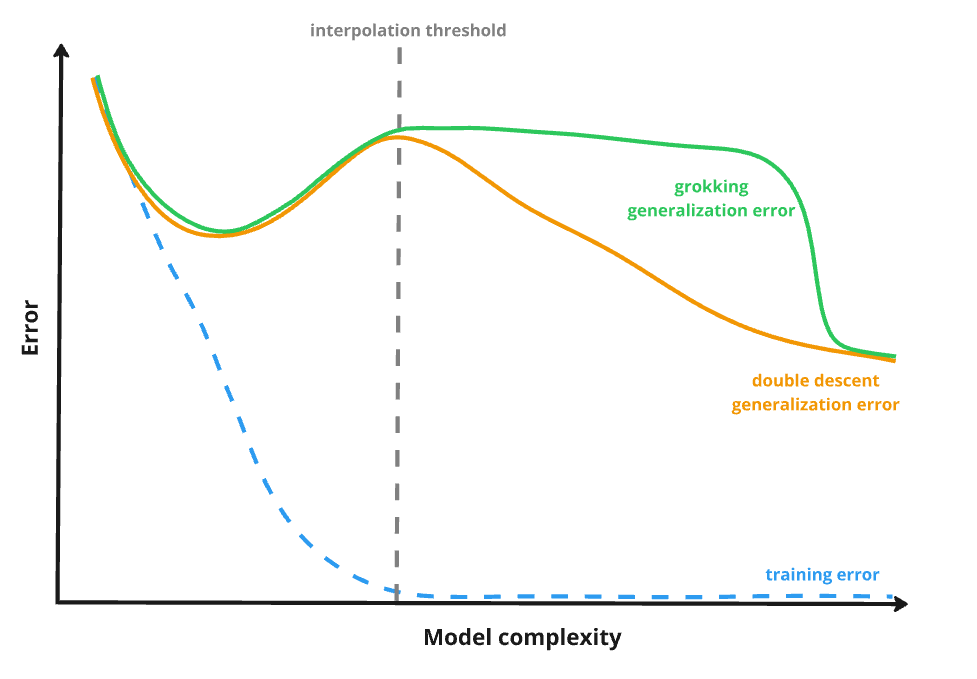
\includegraphics[width=0.6\linewidth]{img/grokking.png}
    \caption[\textit{Grokking} y \textit{Deep Double Descent}.]{Error en entrenamiento y generalización para el caso de \textit{grokking} (línea verde) y para el doble descenso (línea naranja). Se observa que el \textit{grokking} implica una mejora abrupta en términos de generalización una vez superado el umbral de interpolación, mientras que el doble descenso muestra una mejora progresiva a partir de ese punto.}\label{fig:grokking}
\end{figure}

Para concluir este capítulo, se presenta en la Tabla~\ref{tabla:resumen-contribuciones} un resumen de las principales publicaciones relacionadas con el doble descenso, aunque las primeras manifestaciones no utilizan la denominación actual, junto con sus contribuciones más relevantes. Asimismo, se incluye en la tabla el número de citas de cada publicación, obtenido a partir de \textit{Google Scholar}\footnote{Número de citas encontradas a día 14 de marzo de 2025.}.\newline

\begin{table}[h]
    \centering
    \small 
    \renewcommand{\arraystretch}{0.9} 
    \begin{NiceTabular}{c c c c}[hvlines,color-inside]
        \Block[fill={cyan!50}]{2-1}{\textbf{Año}} & \Block[fill={cyan!50}]{2-1}{\textbf{Referencia}} & \Block[fill={cyan!50}]{2-1}{\textbf{Principales contribuciones}} & \Block[fill={cyan!50}]{2-1}{\textbf{Citas}} \\ \\
        
        \Block{3-1}{1989} & \Block{3-1}{Vallet et al.~\cite{Vallet1989}} & \Block{3-1}{Primera manifestación empírica del suceso \\ sobre datos artificiales en la física teórica.} & \Block{3-1}{71} \\ \\ \\

        \Block{3-1}{1991} & \Block{3-1}{Krogh \& Hertz~\cite{Krogh1991}} & \Block{3-1}{Evidenciaron, parcialmente, el fenómeno en el \\ contexto de la regresión lineal.} & \Block{3-1}{2654} \\ \\ \\

        \Block{3-1}{1995} & \Block{3-1}{Manfred Opper~\cite{Opper1995}} & \Block{3-1}{Primeros resultados teóricos formales \\ sobre datos artificiales.} & \Block{3-1}{71} \\ \\ \\

        \Block{3-1}{2000} & \Block{3-1}{Robert Duin~\cite{Duin2000}} & \Block{3-1}{Primeras evidencias empíricas usando \\ datos del mundo real.} & \Block{3-1}{209} \\ \\ \\

        \Block{3-1}{2019} & \Block{3-1}{Belkin et al.~\cite{Belkin2019}} & \Block{3-1}{Unificaron la sabiduría clásica con los enfoques \\ modernos y acuñaron el nombre de \textit{Deep Double Descent}.} & \Block{3-1}{2331} \\ \\ \\

        \Block{3-1}{2019} & \Block{3-1}{Nakkiran et al.~\cite{Nakkiran2019}} & \Block{3-1}{Introdujeron la complejidad efectiva del modelo \\ y los distintos tipos de doble descenso.} & \Block{3-1}{1174} \\ \\ \\

        \Block{3-1}{2021} & \Block{3-1}{Chen et al.~\cite{Chen2021}} & \Block{3-1}{Demostraron que el error puede presentar un \\ número arbitrario de ``picos'' y que pueden controlarse.} & \Block{3-1}{80} \\ \\ \\

        \Block{3-1}{2023} & \Block{3-1}{Schaeffer et al.~\cite{Schaeffer2023}} & \Block{3-1}{Analizaron los factores que provocan su aparición \\ en modelos de regresión polinómica.} & \Block{3-1}{29} \\ \\ \\
    \end{NiceTabular}
    \caption{Resumen de los principales artículos junto con sus contribuciones.}\label{tabla:resumen-contribuciones}
\end{table}

\endinput